\begin{abstract}
Video captions play a crucial role in text-to-video generation tasks, as their quality directly influences the semantic coherence and visual fidelity of the generated videos. Although large vision-language models (VLMs) have demonstrated significant potential in caption generation, existing benchmarks inadequately address fine-grained evaluation, particularly in capturing spatial-temporal details critical for video generation. To address this gap, we introduce the Fine-grained Video Caption Evaluation Benchmark (\textbf{VCapsBench}), the first large-scale fine-grained benchmark comprising 5,677 (5K+) videos and 109,796 (100K+) question-answer pairs. These QA-pairs are systematically annotated across 21 fine-grained dimensions (\eg, camera movement, and shot type) that are empirically proven critical for text-to-video generation. We further introduce three metrics (Accuracy (\textbf{AR}), Inconsistency Rate (\textbf{IR}), Coverage Rate (\textbf{CR})), and an automated evaluation pipeline leveraging large language model (LLM) to verify caption quality via contrastive QA-pairs analysis. By providing actionable insights for caption optimization, our benchmark can advance the development of robust text-to-video models. The dataset and codes are available at website: \url{https://github.com/GXYM/VCapsBench}. 
\end{abstract}

\begin{figure}[ht]
	\begin{minipage}[t]{1.0\linewidth}
        \centering
	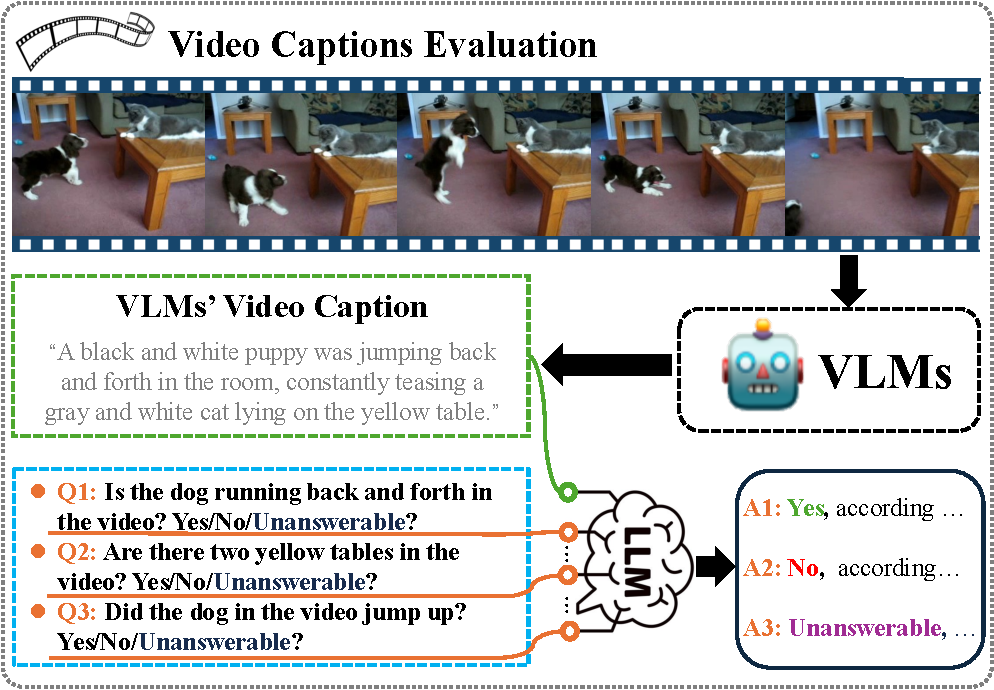
\includegraphics[width=0.8\linewidth]{imgs/intro-2.pdf}
	\caption{Illustration of video caption evaluation by VCapsBench. Evaluate the detail, comprehensiveness, and accuracy of video captions using "yes-no" question-answer pairs.}
	\label{fig:fig1}
	\end{minipage}%
	\vspace{-1.5em}	
\end{figure}